This section presents the results of the different performance tests applied to
a selection of graphical libraries.
The technical characteristics of the computer are:
\begin{itemize}
\item Intel(R) Core(TM)2 Duo CPU 2.66\,[GHz]
\item 4 Gigabyte RAM
\item Operating System Fedora 12 for i686
\end{itemize}

Each benchmark consisted in taking two simple examples
of dynamic data plotting for each library,
in which the \emph{data} was a random value to simulate a real environment.
The tests were repeated
for periods between data updates of 100\,[ms], 10\,[ms] and 1\,[ms]
in each case,
comparing frames per second (FPS) and their variances.
The 100\,[ms] test is slow updates,
10\,[ms] is rather fast and 1\,[ms] is a real stress test.
The scripts running the tests measure the FPS each 200 data objects,
each measurement is one data point in the graphs given below.
Note that raw FPS can be misleading,
for smooth trending graphs 20~FPS is adequate,
while 50~FPS is absolutely perfect.
Perhaps a better measure would be to see how many data points can be updated
at a given rate while still reaching 20~FPS (or 50, as the case may be).
Other considerations are the impact on performance
if there is a clear trend
(new data are just added near the end of the graph)
or appear scattered.
The Data from each plot, come from a method that generates random values,
and the plot refresh is performed using each library's own methods.
The difference between the FPS and the arrived data is that the FPS is
the amount of refresh in the plot, considering the data that have been sent.

\subsection{Java}

Here we compare two Java libraries,
\emph{JFreeChart} and \emph{JChart2D}.
The resulting FPS of each library
for 100\,[ms] are shown in figure~\ref{fig:java100}.
\begin{figure}%[ht]
  \subfigure[{100\,[ms] period}]
  {
    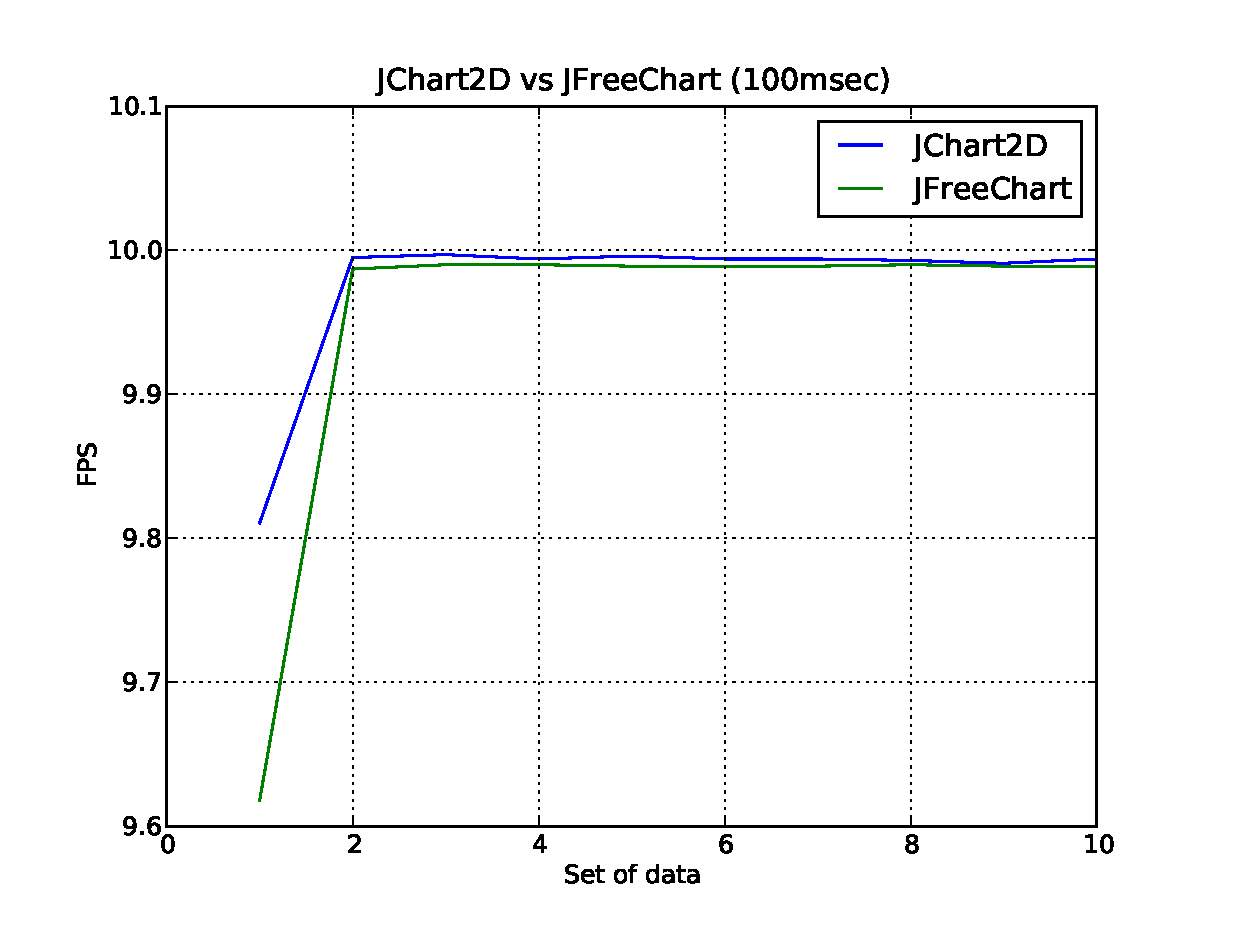
\includegraphics[width=0.32\linewidth, height=!]{../img/java-100}
    \label{fig:java100}
  }
  \subfigure[{10\,[ms] period}]
  {
    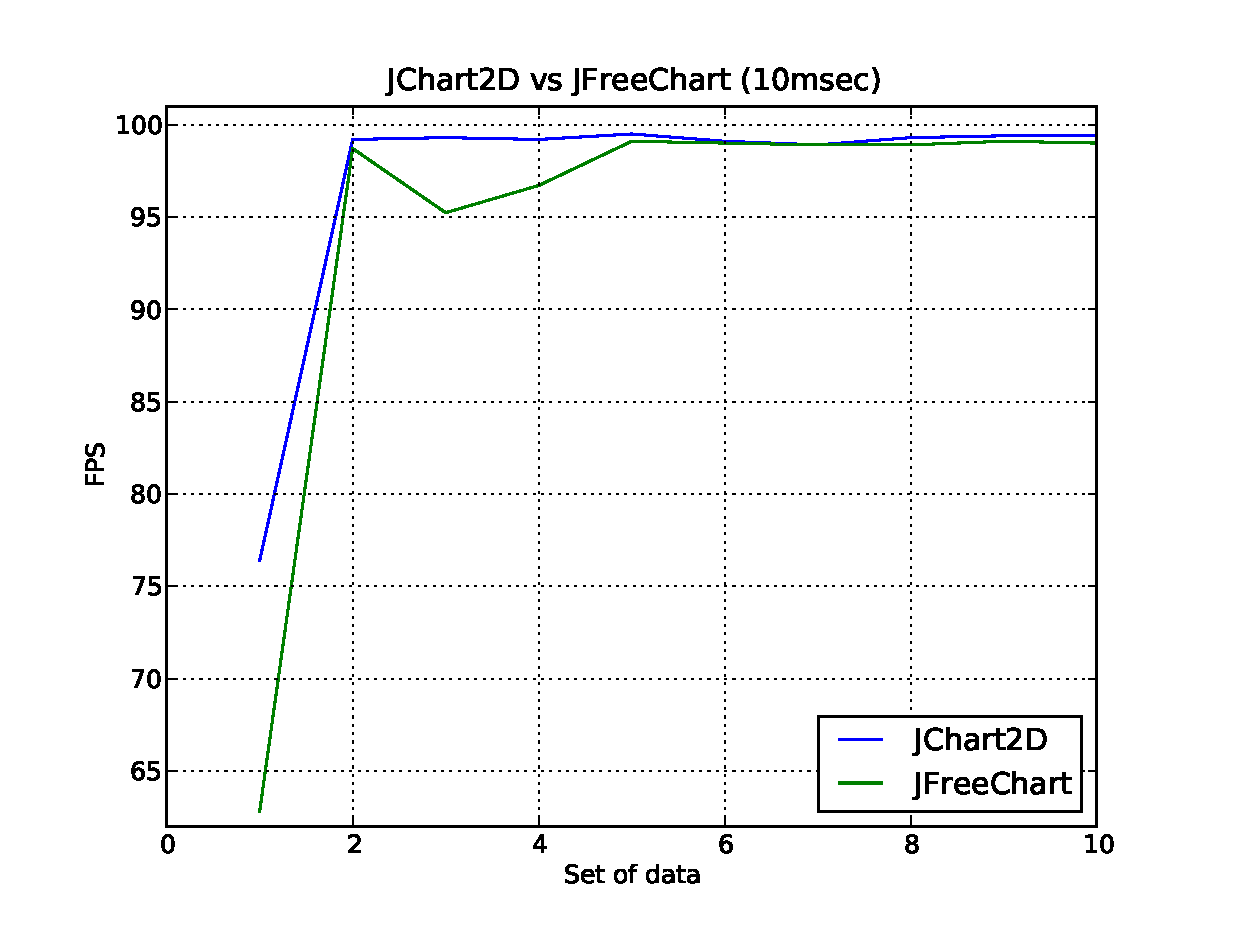
\includegraphics[width=0.32\linewidth, height=!]{../img/java-10}
    \label{fig:java10}
  }
  \subfigure[{1\,[ms] period}]
  {
    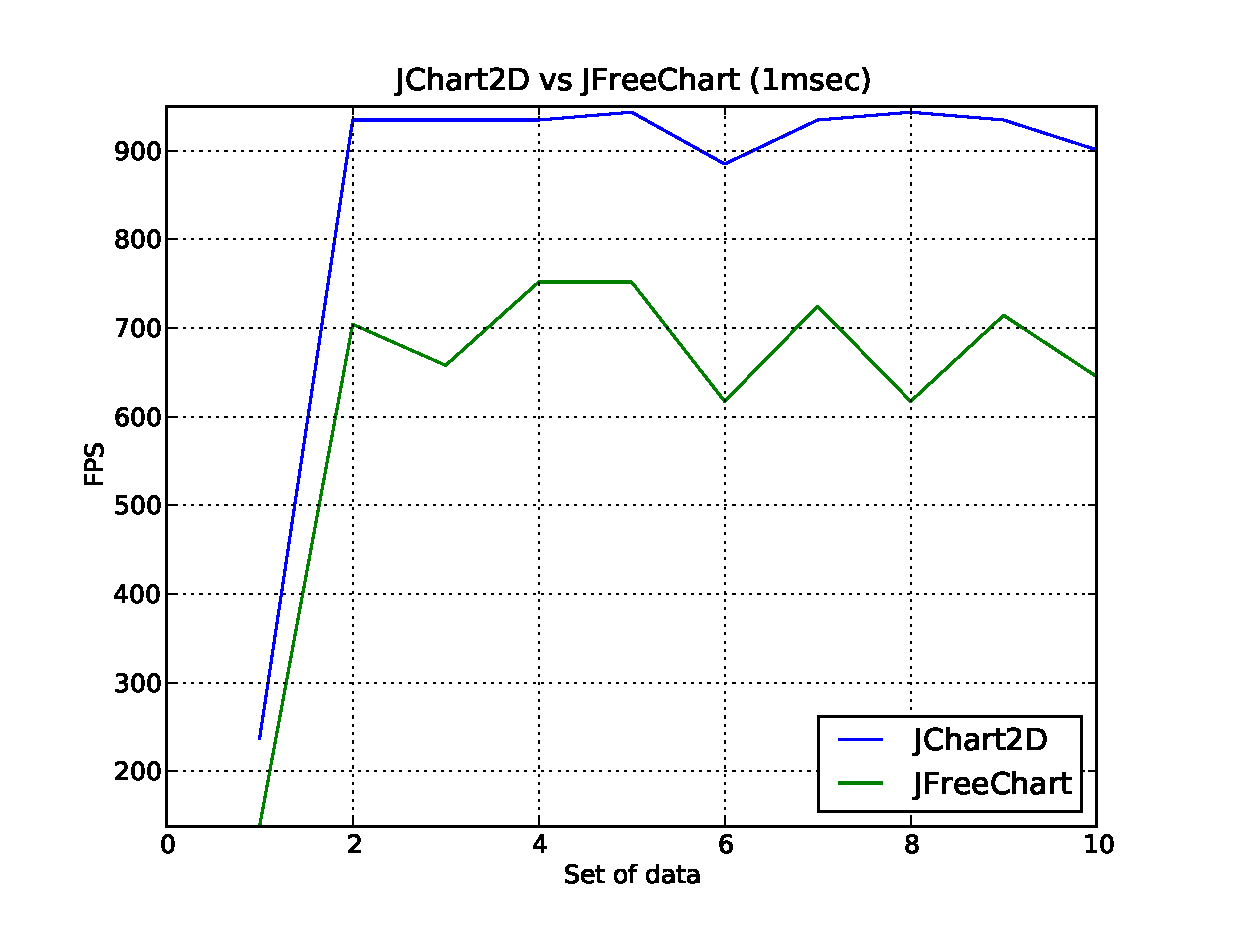
\includegraphics[width=0.32\linewidth, height=!]{../img/java-1}
    \label{fig:java1}
  }
  \label{fig:figure1}
  \caption{JChart2D and JFreeChart comparison plots}
\end{figure}
At first look, JFreeChart shows a inconspicuous lower performance graphing data
with 100\,[ms] of latency time.
There is little difference between the averages
of each library, of the order of $0.024$.
JChart2D has a standard deviation of $0.055$ and a average of $9.975$, which means that
the difference between the FPS are very similar, and has a minimal variation.
JFreeChart has a standard deviation of $0.111$ and a average of $9.952$, which means that
the difference between the FPS at each point has a minimal variation, but is higher compared
to JChart2D.
An important fact is that this latency is slow, so taking it as
reference the scientific data visualization topic we need receiving the data
with a higher frequency.

The second test was performed with an interval of 10\,[ms],
giving the results in figure~\ref{fig:java10}
Decreasing the interval ten times
we see that the difference between the averages of the libraries
increases a little more, we are talking about $2.22$ frames more
for JChart2D.
JChart2D has a standard deviation of $6.861$ and a average of $96.974$, which means that
the difference between the FPS are now higher than in the previous test,
ant it is a large for this same task.
JFreeChart has a standard deviation of $10.717$ and a average of $94.754$, which means that
the difference between the FPS at each point has a noticeable variation, and is higher than the one exhibited by JChart2D.
Also, JChart2D has a regular performance varying a little at each
point, but JFreeChart does not have a regular performance, the three
and four points showed a substantial fall. This fact makes this library unsuitable,
because visualizing scientific data requires a regular
expected behavior.

The third test was performed with a latency time of 1\,[ms].
The resulting FPS of each library are shown in figure~\ref{fig:java1}.
Finally, the difference between FPS for each library
is more noticeable, we are talking about $225.98$ FPS,
and JChart2D outperforms JFreeChart.
JChart2D has a standard deviation of $207.715$ and a average of $858.307$, which means that
the difference between the FPS are now higher related to the two previous tests,
we also note that as the FPS at each point are large values in comparison, so that implies
the big difference between the values.
JFreeChart has a standard deviation of $171.445$ and a average of $632.322$, which means that
this library has a lower standard deviation related to the JChart2D, but the value still being
a large value for a standard deviation; in another hand, the average has a lower value related
the JChart2D average.
Like the previous test, we can look the irregularities of the
JFreeChart performance, at points 3,6, 8 and 10,
so this reaffirms the previous fact that the performance
of JChart2D is most recommendable.

\subsection{Python}

We also compared two Python libraries,
\emph{PyQwt} and \emph{Matplotlib}.
First, the programs start with an interval of data actualization of 100\,[ms],
and the resulting FPS of each library are shown in figure~\ref{fig:python100}.
In this test, as we know in the case of Java, is a kind of non realistic test,
because the data was actualized slowly.
PyQwt has a more stable performance, showing a standard deviation of $0.0004$ that is very close to zero,
keeping the FPS near to 10, but the average of $9.999$ is lower in relation to Matplotlib.
In the side of Matplotlib, the performance has higher and lower points,
but at point number 4 it stabilizes, having an average close to $10.029$.
At first look, Matplotlib is a better choice because it has a better average, but a higher standard variation, $0.010$;
but if the programmer is looking for a library with stable performance,
choosing Matplotlib means taking some risks.

Second, the programs start with an interval of data actualization of 10\,[ms],
and the resulting FPS of each library are shown in figure~\ref{fig:python10}
\begin{figure}%[ht]
  \subfigure[{100\,[ms] period}]{
    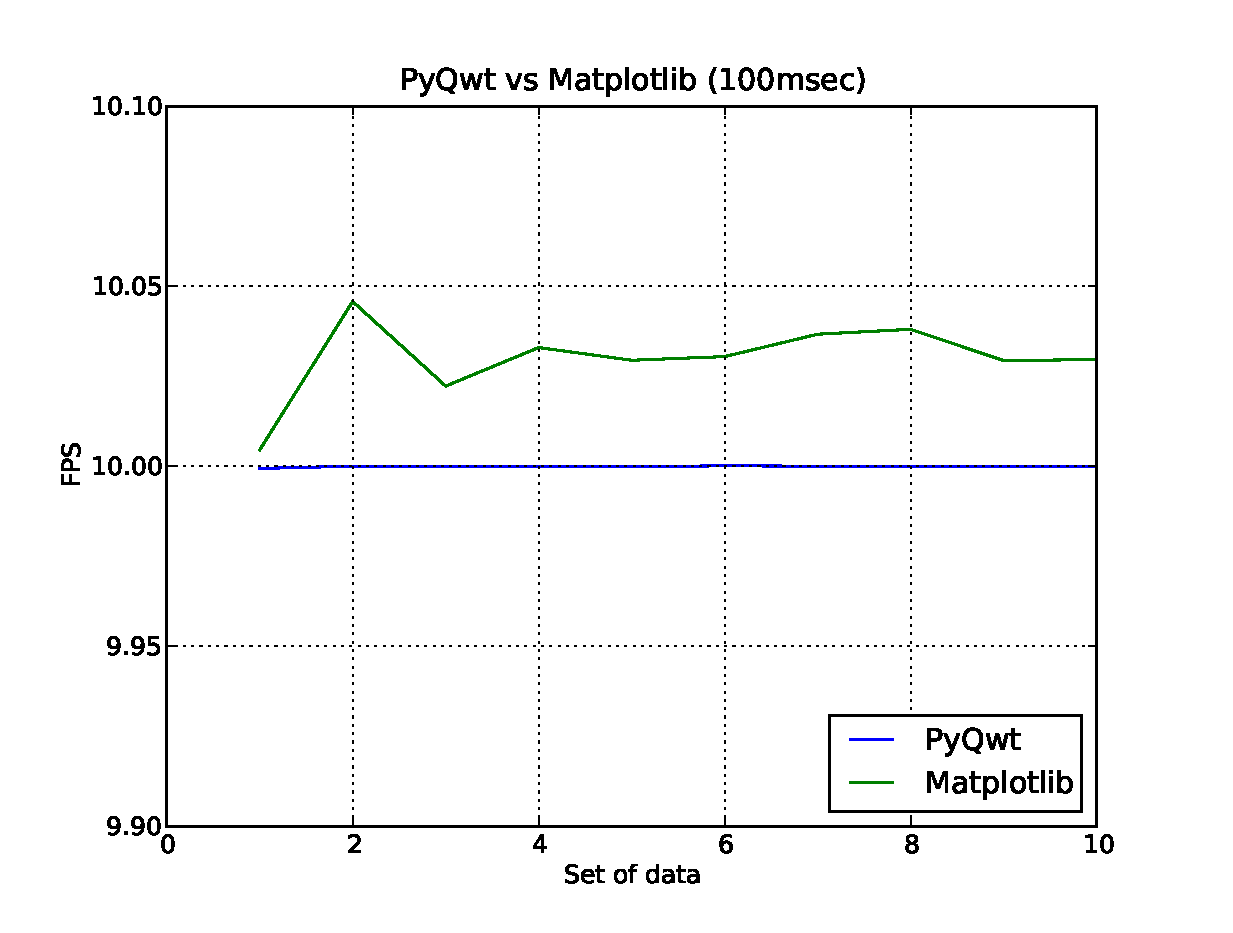
\includegraphics[width=0.32\linewidth, height=!]{../img/python-100}
    \label{fig:python100}
  }
  \subfigure[{10\,[ms] period}]{
    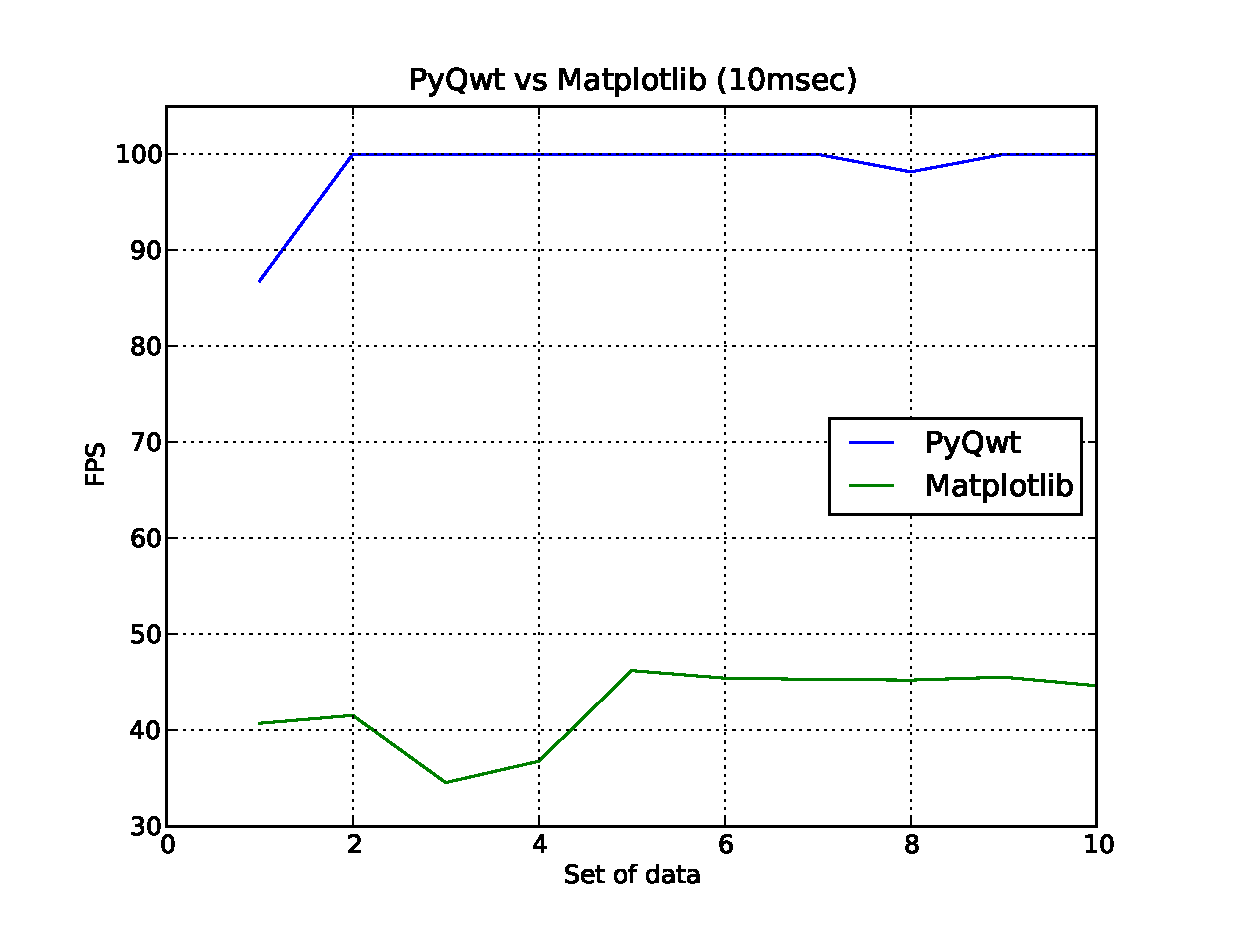
\includegraphics[width=0.32\linewidth, height=!]{../img/python-10}
    \label{fig:python10}
  }
  \subfigure[{1\,[ms] period}]{
    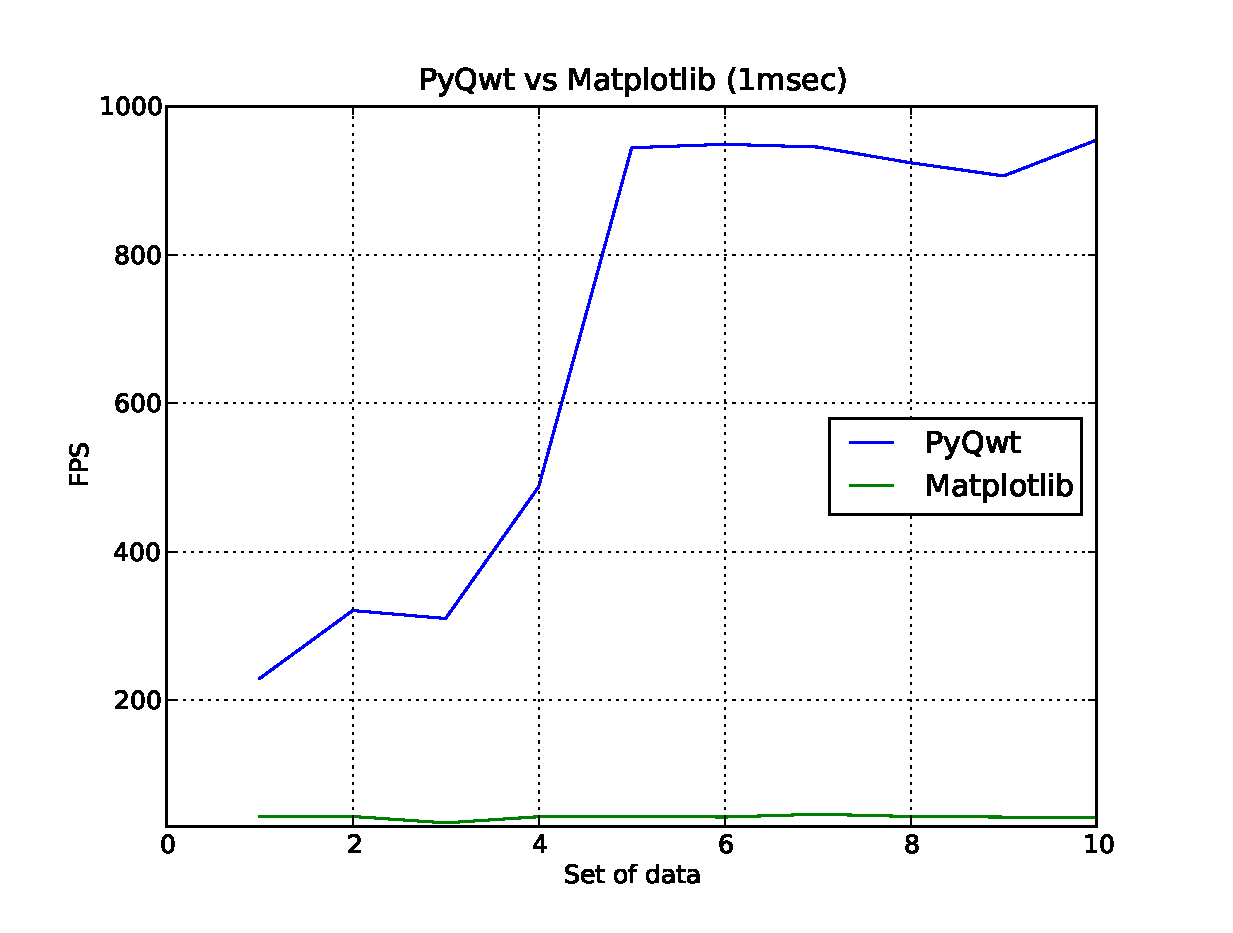
\includegraphics[width=0.32\linewidth, height=!]{../img/python-1}
    \label{fig:python1}
  }
  \label{fig:figure3}
  \caption{PyQwt and Matplotlib comparison plots}
\end{figure}
In this test, a notorious difference comes out,
because the difference between the averages is around $55.90$
FPS, so PyQwt library is the best choice with a average of $98.500$.
Anyway, Matplotlib tries to gain performance from point 5 on forward, but still having
a lower average of $42.598$.
The standard variation of these libraries are very  similar, being $3.932$ and $3.887$ relatively.
On the other hand, the PyQwt has a more constant performance,
which tell us the stability of the library.

Third, the programs start with an interval of data actualization of 1\,[ms],
and the resulting FPS of each library are as given in figure~\ref{fig:python1}.
In this stressed situation the notorious
difference between the performance of PyQwt and Matplotlib
is finally visible,
showing averages of $697.050$ and $42.463$, respectively.
Aside of the performance average, the standard deviation of Matplotlib of $2.809$ is
much lower compared to the PyQwt standard deviation of $300.325$, but this has
direct relation with the obtained values at each point.
As final words it is necessary to say that Matplotlib is not
designed purely to create dynamic plots, its main goal
is to create a lot of graph types in a easy way~\cite{matplotlib-paper}.
On the other hand, PyQwt has the direct binding from the Qwt library
that was designed to obtain high performance in data trending.

\subsection{C++}

Finally, on the C++ side we present the  results of the comparison between
\emph{Qwt} and \emph{wxMathPlot}.
The thread handling in C++ is more efficient,
as it isn't hindered by portability layers.
As a result,
the FPS values obtained are much larger than the ones in previous tests.
FPS in this case are almost equivalent to the data generation rate.

First, the programs start with an interval of data actualization of 100\,[ms] (latency time),
and the resulting \emph{Frames Per Second (FPS)} of each library are shown in figure~\ref{fig:c++100}
\begin{figure}%[ht]
  \subfigure[{100\,[ms] period}]{
    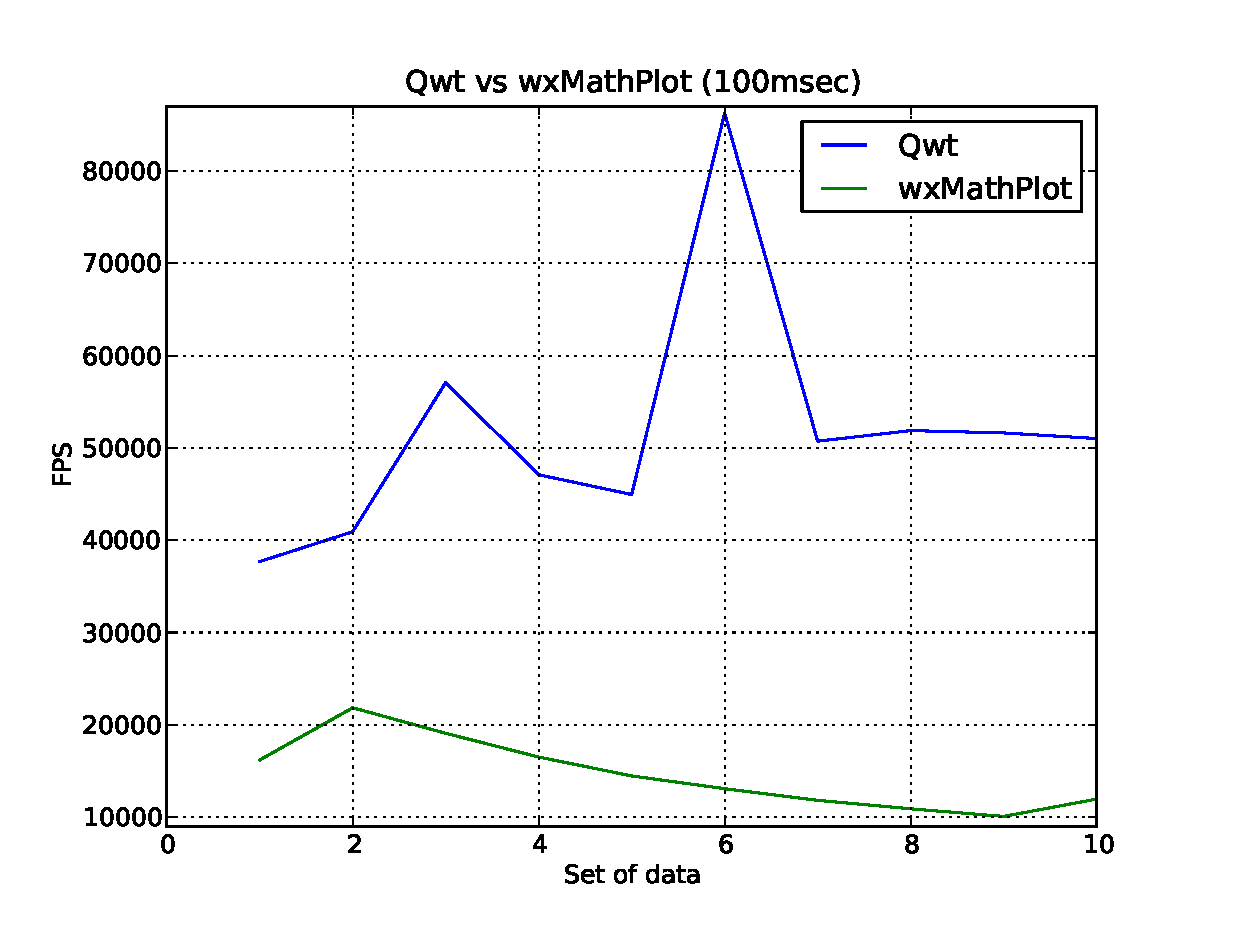
\includegraphics[width=0.32\linewidth, height=!]{../img/c++-100}
    \label{fig:c++100}
  }
  \subfigure[{10\,[ms] period}]{
    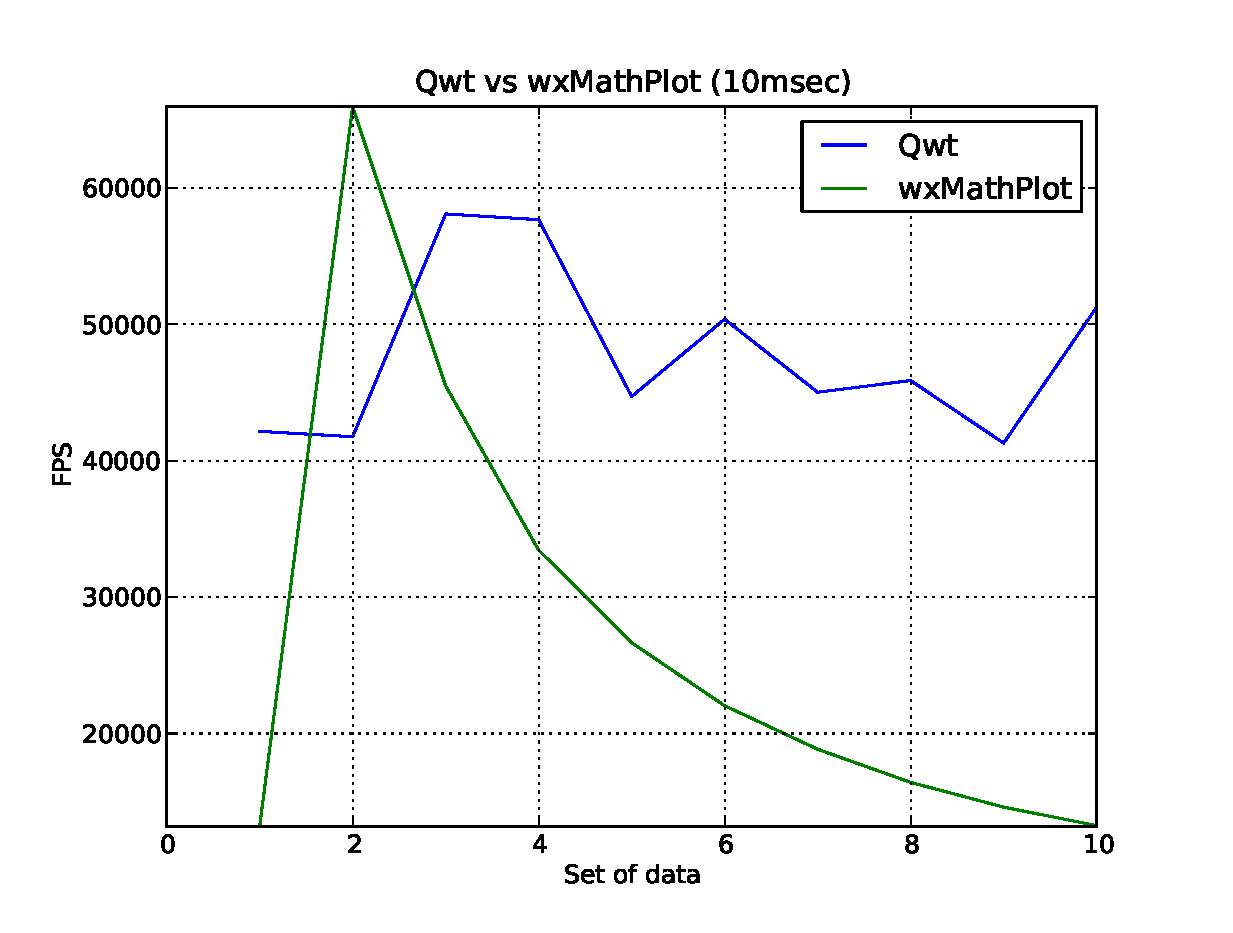
\includegraphics[width=0.32\linewidth, height=!]{../img/c++-10}
    \label{fig:c++10}
  }
  \subfigure[{1\,[ms] period}]{
    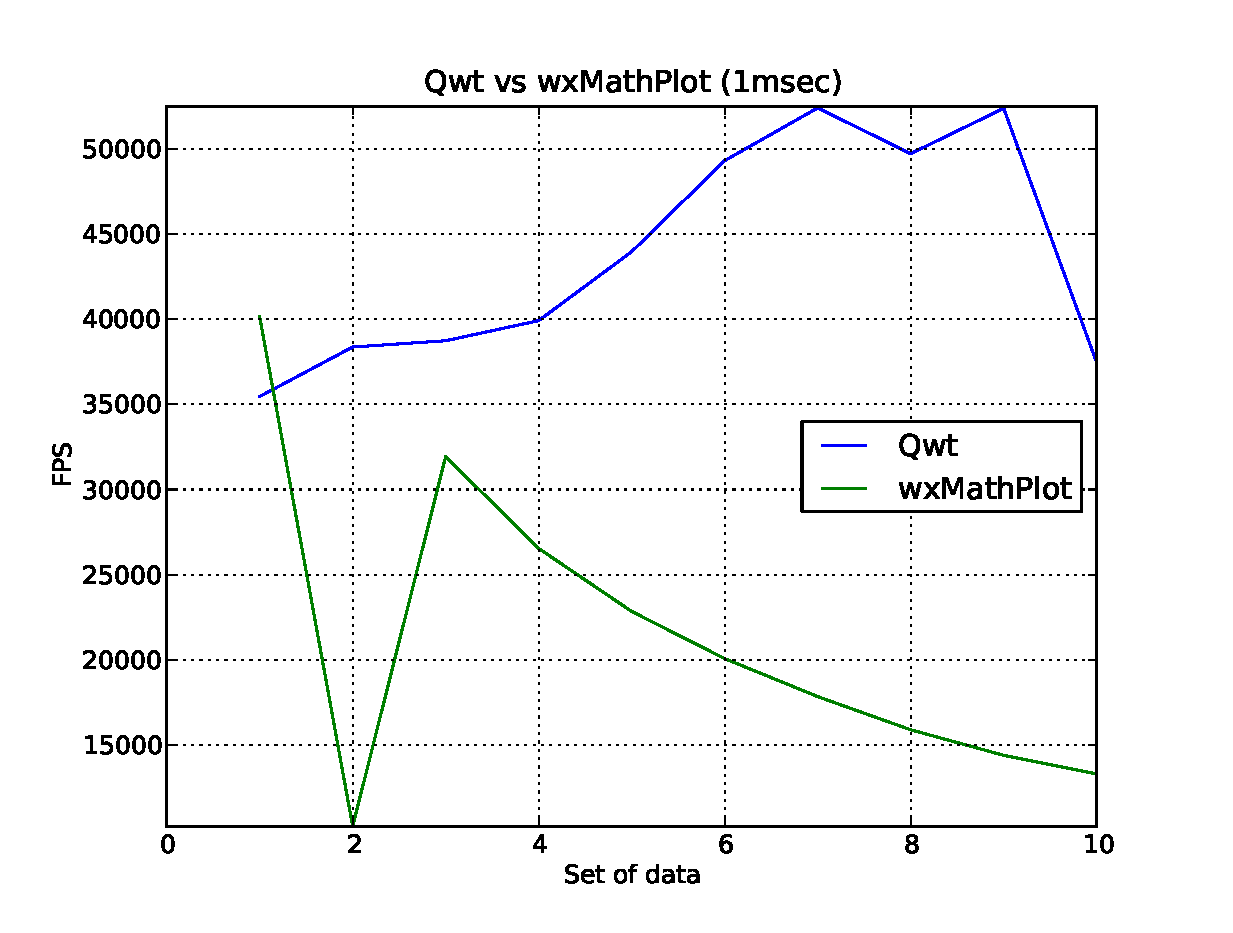
\includegraphics[width=0.32\linewidth, height=!]{../img/c++-1}
    \label{fig:c++1}
  }
  \label{fig:figure4}
  \caption{Qwt and wxMathPlot comparison plots}
\end{figure}
The Qwt library shows better performance than wxMathPlot,
which is reflected in the average of each, $51916.5$ and $14589.5$,
respectively.
On the other hand, the standard deviation tells us about the stability
of each library, in this case wxMathPlot has a decreasing stability,
with a standard deviation of $3605.235$, which is acceptable because
the quantity of data is large enough. Also the Qwt library,
has a more unstable behavior with higher and lower points,
which is defined by their standard deviation of $51916.5$ that is
greater that the previous by one order of magnitude.

Continuing with the test, now with a latency rate of 10\,[ms],
the results in FPS are in figure~\ref{fig:c++10}.
In this case the Qwt performance increases a little, but at
point 2 for example, it is surpassed by wxMathPlot. But in general,
Qwt has better performance with a average of $47830.2$ in
comparison to the $26988.1$ of wxMathPlot.
Respect to the standard deviation wxMathPlot remains the
decreasing stability showing a value of $16242.412$,
that is very high in relation with the standard deviation of
Qwt, $5949.169$. Also Qwt still shows an irregularity
in its performance, due to thread behavior.

Finally we have the last test, that consist in stressing out C++ data trending, with a latency time of 1\,[ms].
The results are in the figure~\ref{fig:c++1}.
In this test, both libraries show very strange behavior, due to the
data Thread actualization with a very low value as is 1\,[ms].
Qwt still wins the match with wxMathPlot, but the irregularity is still present,
because the standard deviation raises to $6271.181$, but in the case of wxMathPlot
that value decreases to $8805.198$, which means that in stability wxMathPlot has the
first place, but related to performance, Qwt wins with a average of $43771.6$
over the wxMathPlot average of $21316.9$.


\subsection{General comments}

The reasons of the lower performance of Python and Java wit respect to C++
are very simple to explain. The execution of every Java program depends on the
Java Virtual Machine.
With respect to Python, PyQwt has simple bindings to the Qwt/C++ library, so they
have a longer path to walk to interact with the final plot.

Another important issue is the threads implementation of each language.
The C++ Standard Library has less features (functionality) and a limited scope
related to the Java Standard Library, but includes native threads libraries.
On the other hand, Python provides low-level primitives for working with multiple threads,
but in difference to C++, Python has POSIX threads and non-POSIX threads.

Software developed in Python is generally slower than Java,
but development time is less with Python,
since Python has dynamic typing and offers built-in high-level data types.
Comparing Java with C++ brings us to similar conclusions.
